% !TeX root = ../main.tex

\newlecture[Duration for Bond Portfolios \& Immunization][Oct 8, 2026]

\header{Duration of a Portfolio}
\begin{definition}[\rb{Portfolio Duration}]
    Given fixed income securities with prices $P_i$ and durations $D_i$, $i = 1, \dots, m$, the portfolio consisting of the aggregate of these has price $P$ and duration $D$:
    \[\boxed{\begin{gathered}
        P = P_1 + P_2 + \cdots + P_m\\
        D = w_1D_1 + w_2D_2 + \cdots + w_mD_m, \qquad w_i = \frac{P_i}{P}
    \end{gathered}}\]
    Works for both \dbb{Macaulay} and \dbb{all forms of modified} duration.
\end{definition}
\keypoint{\db{Note}: this looks just like the Macaulay duration formula, except with \rb{time replaced by duration}!\\(Weights are each security's share of the total price.)}

\heading{Derivation}
Take two cash flow streams $A$ and $B$ over the same times $t_0, \dots, t_n$ (a stream with no payment at $t_k$ just has $PV_k = 0$ there):
\begin{center}
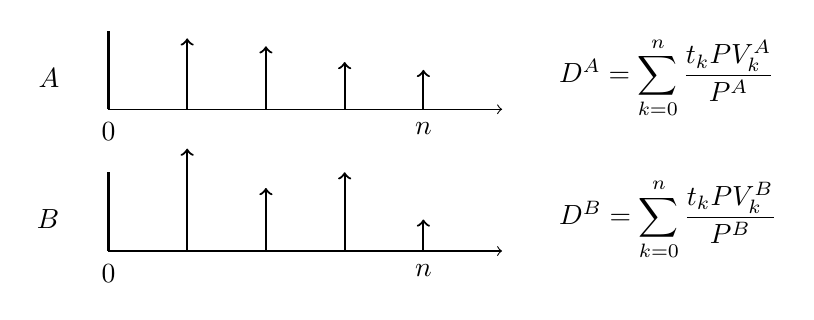
\begin{tikzpicture}
    \foreach \row/\lab/\hs in {0/A/{0.9,0.8,0.6,0.5}, -1.8/B/{1.3,0.8,1.0,0.4}} {
        \begin{scope}[yshift=\row cm]
            \node[left] at (-0.5,0.4) {$\lab$};
            \draw[->] (0,0) -- (5,0);
            \draw[thick] (0,0) -- (0,1.0);
            \node[below] at (0,-0.05) {$0$};
            \node[below] at (4,-0.05) {$n$};
            \foreach \h [count=\k] in \hs { \draw[->, thick] (\k,0) -- (\k,\h); }
            \node[right] at (5.6,0.4) {$D^{\lab} = \displaystyle\sum_{k=0}^{n}\frac{t_k PV_k^{\lab}}{P^{\lab}}$};
        \end{scope}
    }
\end{tikzpicture}
\end{center}
The duration of $A + B$ (cash flows add, so PVs add):
\begin{align*}
    D^{A+B} &= \sum_{k=0}^{n}\frac{t_k\left(PV_k^A + PV_k^B\right)}{P^A + P^B}
    = \sum_{k=0}^{n}\frac{t_kPV_k^A}{P^A + P^B} + \sum_{k=0}^{n}\frac{t_kPV_k^B}{P^A + P^B}\\
    &= \sum_{k=0}^{n}\frac{t_kPV_k^A}{P^A + P^B}\cdot\textcolor{red!70!black}{\frac{P^A}{P^A}} + \sum_{k=0}^{n}\frac{t_kPV_k^B}{P^A + P^B}\cdot\textcolor{red!70!black}{\frac{P^B}{P^B}} && \text{(multiply by 1)}\\
    &= \underbrace{\sum_{k=0}^{n}\frac{t_kPV_k^A}{\textcolor{red!70!black}{P^A}}}_{D^A}\left(\frac{\textcolor{red!70!black}{P^A}}{P^A + P^B}\right) + \underbrace{\sum_{k=0}^{n}\frac{t_kPV_k^B}{\textcolor{red!70!black}{P^B}}}_{D^B}\left(\frac{\textcolor{red!70!black}{P^B}}{P^A + P^B}\right) && \text{(swap denominators)}
\end{align*}
\[\boxed{D^{A+B} = \left(\frac{P^A}{P^A + P^B}\right)D^A + \left(\frac{P^B}{P^A + P^B}\right)D^B = w_AD^A + w_BD^B}\]
The weights add to 1 ($w_A + w_B = 1$), so $D^{A+B}$ always lies \ul{between} $D^A$ and $D^B$ (for positive prices). Repeating this for more streams gives the general formula.
\\Note: the derivation needs every $PV_k$ to be computed with the \ul{same rate} (one common yield, or one spot rate curve). If the bonds have different yields, the formula is only an approximation.

\header{Immunization}
\begin{definition}[\rb{Immunization}]
    Constructing a portfolio of bonds which is \dbb{protected (immunized) against changes in interest rates}.
\end{definition}

\b{Problem}: you have an obligation to pay \$1,000 two years from now, but you can only purchase bonds of maturity 1 and 5 years.
\begin{itemize}
    \item 1 year bond only: \dbb{reinvestment risk}. The money must be reinvested at year 1 at an unknown future rate.
    \item 5 year bond only: \dbb{too sensitive to interest rates}. It must be sold at year 2 at an unknown price.
\end{itemize}

\begin{center}
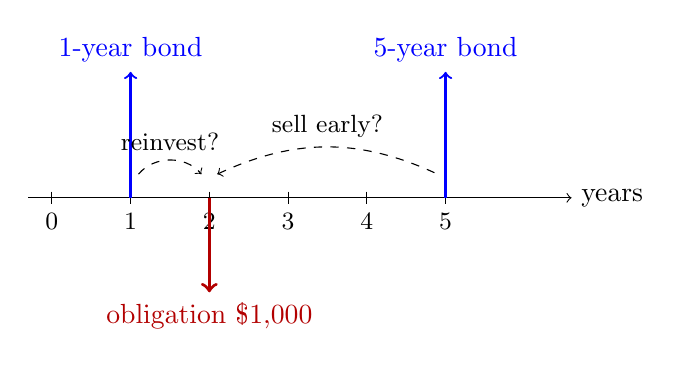
\begin{tikzpicture}
    \draw[->] (-0.3,0) -- (6.6,0) node[right] {years};
    \foreach \x in {0,...,5} { \draw (\x,0.08) -- (\x,-0.08) node[below] {\small \x}; }
    \draw[->, very thick, red!70!black] (2,0) -- (2,-1.2) node[below] {obligation \$1,000};
    \draw[->, thick, blue] (1,0) -- (1,1.6) node[above] {1-year bond};
    \draw[->, thick, blue] (5,0) -- (5,1.6) node[above] {5-year bond};
    \draw[->, dashed] (1.1,0.3) to[bend left=50] node[above] {\small reinvest?} (1.9,0.3);
    \draw[<-, dashed] (2.1,0.3) to[bend left=25] node[above] {\small sell early?} (4.9,0.3);
\end{tikzpicture}
\end{center}

\keypoint{\rb{Solution}: construct a portfolio of 1 and 5 year securities with the same \rb{present value} and \rb{duration} as your obligation.}

With $x$ units of bond 1 (price $P_1$, duration $D_1$) and $y$ units of bond 2 (price $P_2$, duration $D_2$), and an obligation with present value $P$ and duration $D$:
\[\boxed{\begin{aligned}
    \text{PV:} &\quad xP_1 + yP_2 = P\\
    \text{Duration:} &\quad \frac{xP_1}{P}D_1 + \frac{yP_2}{P}D_2 = D
\end{aligned}}\]
Solve these two equations for $x$ and $y$ to determine your portfolio. The duration equation is just the portfolio duration formula, with weights $w_1 = \frac{xP_1}{P}$ and $w_2 = \frac{yP_2}{P}$.

\b{Why it works}: equal PV means equal value \ul{now}. Equal duration means equal $\frac{dP}{d\lambda}$ (since $\frac{dP}{d\lambda} = -D_mP$), so when the yield moves a little, the portfolio and the obligation \ul{change in value by about the same amount}. The portfolio can still cover the obligation.

\begin{example}
    You have an obligation of \$1,000 in 2 years, and wish to invest now to meet it. You can invest in 1 year and 5 year zero-coupon bonds (face \$100, discrete yearly compounding, yield 9\%):
    \begin{center}
    \begin{tabular}{lccccc}
        \toprule
        & Coupon & Maturity & Yield & Price & Duration (Mac)\\
        \midrule
        \textcolor{red!70!black}{Obligation} & \multicolumn{3}{c}{\textcolor{red!70!black}{\$1,000 in 2 years}} & \textcolor{red!70!black}{\$841.68} & \textcolor{red!70!black}{2 years}\\
        \db{Bond 1} & 0\% & 1 year & 9\% & \$91.74 & 1 year\\
        \db{Bond 2} & 0\% & 5 years & 9\% & \$64.99 & 5 years\\
        \bottomrule
    \end{tabular}
    \end{center}
    Prices: $\frac{1000}{1.09^2} = 841.68$, $\frac{100}{1.09} = 91.74$, $\frac{100}{1.09^5} = 64.99$. Each is a zero, so its Macaulay duration is its maturity.
    \\Let $x$ = number of bond 1, $y$ = number of bond 2 held.
    \begin{align*}
        \text{Match prices:} &\quad 91.74x + 64.99y = 841.68\\
        \text{Match durations:} &\quad \frac{91.74x}{841.68}(1\text{ year}) + \frac{64.99y}{841.68}(5\text{ years}) = 2\text{ years}
    \end{align*}
    Multiplying the duration equation by 841.68 and subtracting the price equation: $4(64.99)y = 841.68$, so
    \[\boxed{x = 6.88, \quad y = 3.24}\]
    In weights, $w_1 + w_2 = 1$ and $w_1(1) + w_2(5) = 2$ give $w_1 = \frac{3}{4}$ and $w_2 = \frac{1}{4}$. So \$631.26 goes into bond 1 and \$210.42 into bond 2.
\end{example}

\begin{example}[Bond Immunization Spreadsheet]
    Yield 9\% (semi-annual compounding, 4.5\% per period). Obligation of \$1,000,000 in 10 years, to be immunized using:
    \begin{center}
    \begin{tabular}{lcccccc}
        \toprule
        & Maturity & Principal & Coupon & Price & Macaulay $D$ & \$ amount\\
        \midrule
        Bond 1 & 20 & \$1,000 & 4\% & \$539.96 & 11.45191 & \$321,333.61\\
        Bond 2 & 5 & \$1,000 & 0\% & \$643.93 & 5 & \$93,309.25\\
        \midrule
        Obligation & 10 & \$1,000,000 & 0\% & \$414,642.86 & 10 & \$414,642.86\\
        \bottomrule
    \end{tabular}
    \end{center}
    \begin{itemize}
        \item Prices at 4.5\% per period, e.g.\ bond 2: $\frac{1000}{1.045^{10}} = 643.93$, obligation: $\frac{1{,}000{,}000}{1.045^{20}} = 414{,}642.86$.
        \item Match durations with weights: $11.45191\,w_1 + 5(1 - w_1) = 10 \;\Rightarrow\; w_1 = \frac{5}{6.45191} = 0.775$.
        \item \$ amounts: $0.775(414{,}642.86) = \$321{,}333.61$ in bond 1, and the rest, \$93,309.25, in bond 2.
        \item Number of bonds $= \frac{\$\text{ amount}}{\text{price}}$: \dbb{595.1059} of bond 1 and \dbb{144.9064} of bond 2.
    \end{itemize}
    Note the target duration (10) must lie \ul{between} the two bonds' durations (5 and 11.45). Otherwise one weight is negative, i.e.\ a short position.
\end{example}

\header{The Real Idea Behind Immunization: Taylor Expansions!}
With $\lambda_0$ the current value of the yield, expand the price as a function of the yield around the current value:
\[\boxed{P(\lambda) = \underset{\mathclap{\substack{\Big\uparrow\\\text{price}}}}{P(\lambda_0)} + \underbrace{P'(\lambda_0)(\lambda - \lambda_0)}_{\text{duration}} + \underbrace{\tfrac{1}{2}P''(\lambda_0)(\lambda - \lambda_0)^2}_{\text{convexity}} + \cdots}\]
Here duration and convexity are \dbb{unnormalized}: $P'(\lambda_0) = -D_mP(\lambda_0)$ is modified duration times price.

\keypoint{You can match as many terms as you like to make the Taylor series of your portfolio look like the Taylor series of your cash flow stream (obligation).}

\begin{itemize}
    \item Matching \b{PV and duration} (as above) matches the first two terms. The portfolio and obligation price-yield curves are \dbb{tangent} at $\lambda_0$.
    \item Matching \b{convexity} too would match the curvature, but needs a third equation, so a third bond.
\end{itemize}

\begin{center}
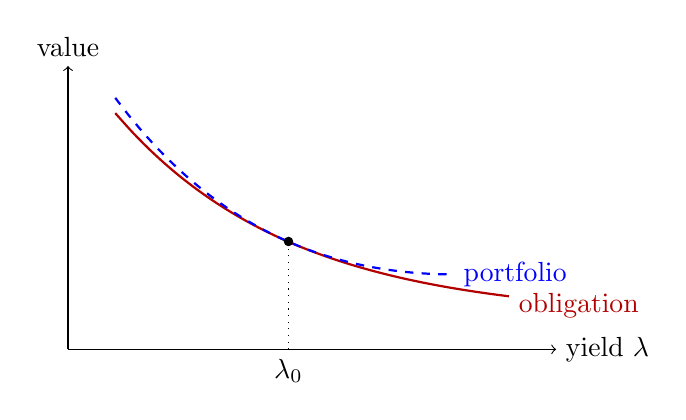
\begin{tikzpicture}
    \draw[->] (0,0) -- (6.2,0) node[right] {yield $\lambda$};
    \draw[->] (0,0) -- (0,3.6) node[above] {value};
    \draw[thick, red!70!black, domain=0.6:5.6, smooth, variable=\x] plot ({\x}, {0.4 + 2.6*exp(-0.45*(\x-0.6))});
    \draw[thick, blue, dashed, domain=0.6:4.9, smooth, variable=\x] plot ({\x}, {0.4 + 2.6*exp(-0.45*(\x-0.6)) + 0.04*(\x-2.8)^2});
    \draw[dotted] (2.8,0) -- (2.8,1.37);
    \node[below] at (2.8,0) {$\lambda_0$};
    \filldraw (2.8,1.37) circle (1.5pt);
    \node[red!70!black, right] at (5.6,0.55) {obligation};
    \node[blue, right] at (4.9,0.95) {portfolio};
\end{tikzpicture}
\end{center}
Same value and slope at $\lambda_0$, so small yield changes affect both equally. For larger changes, the curvature (convexity) difference shows up.
